% !TeX root = PA_QA_Report_Validation.tex
% !TeX program = pdflatex
\documentclass[11pt,a4paper]{article}

\pdfminorversion=7

% ── Packages ──
\usepackage[top=0.9in,left=0.9in,right=0.9in,bottom=1.2in]{geometry}
\usepackage{array}
\usepackage{ragged2e}
\usepackage{setspace}
\usepackage{hyperref}
\usepackage{enumitem}
\usepackage{graphicx}
\usepackage{eso-pic}
\usepackage{fancyhdr}
\usepackage{tabularx}
\usepackage{float}
\usepackage{xcolor}
\usepackage{parskip}
\usepackage{colortbl}
\usepackage{longtable}
\usepackage{caption}
\usepackage{bookmark}

% ── Font (Helvetica / Arial-like, matching SRS) ──
\usepackage[T1]{fontenc}
\usepackage[scaled=0.95]{helvet}
\renewcommand{\familydefault}{\sfdefault}
\setstretch{1.0}
\frenchspacing

% ── Colours ──
\definecolor{tableheader}{RGB}{240, 240, 240}
\definecolor{tablerow}{RGB}{250, 250, 250}

% ── Hyperref setup ──
\hypersetup{
    colorlinks=true,
    linkcolor=blue,
    urlcolor=blue,
    citecolor=blue,
    pdfauthor={Paragon Assurance},
    pdftitle={AI Review -- QA Report Validation},
}

% ── Compact spacing ──
\setlength{\parskip}{0.4em}
\setlist{nosep, leftmargin=1.5em}

% ── Global table row height ──
\renewcommand{\arraystretch}{1.4}

% ── Header/Footer ──
\pagestyle{fancy}
\fancyhf{}
\lhead{\textbf{Paragon Assurance}}
\rhead{QA Report Validation Review}
\cfoot{\thepage}
\renewcommand{\headrulewidth}{0.4pt}
\setlength{\headheight}{20pt}

% ── Column type for wrapped text ──
\newcolumntype{L}[1]{>{\RaggedRight\arraybackslash}p{#1}}

% ── Document ──
\begin{document}

% ══════════════════════════════════════════════════════════════
% Cover Page
% ══════════════════════════════════════════════════════════════
\thispagestyle{empty}
\fancyhf{}
\lhead{}
\rhead{}
\cfoot{}
\renewcommand{\headrulewidth}{0pt}

\newgeometry{top=4.5cm,left=0.9in,right=0.9in,bottom=1.2in}

% ── Letterhead for cover page only ──
\AddToShipoutPictureBG*{%
  \AtPageLowerLeft{%
    
\includegraphics[width=\paperwidth,height=\paperheight]{Paragon_Letterhead.pdf}%
  }%
}

\begin{center}
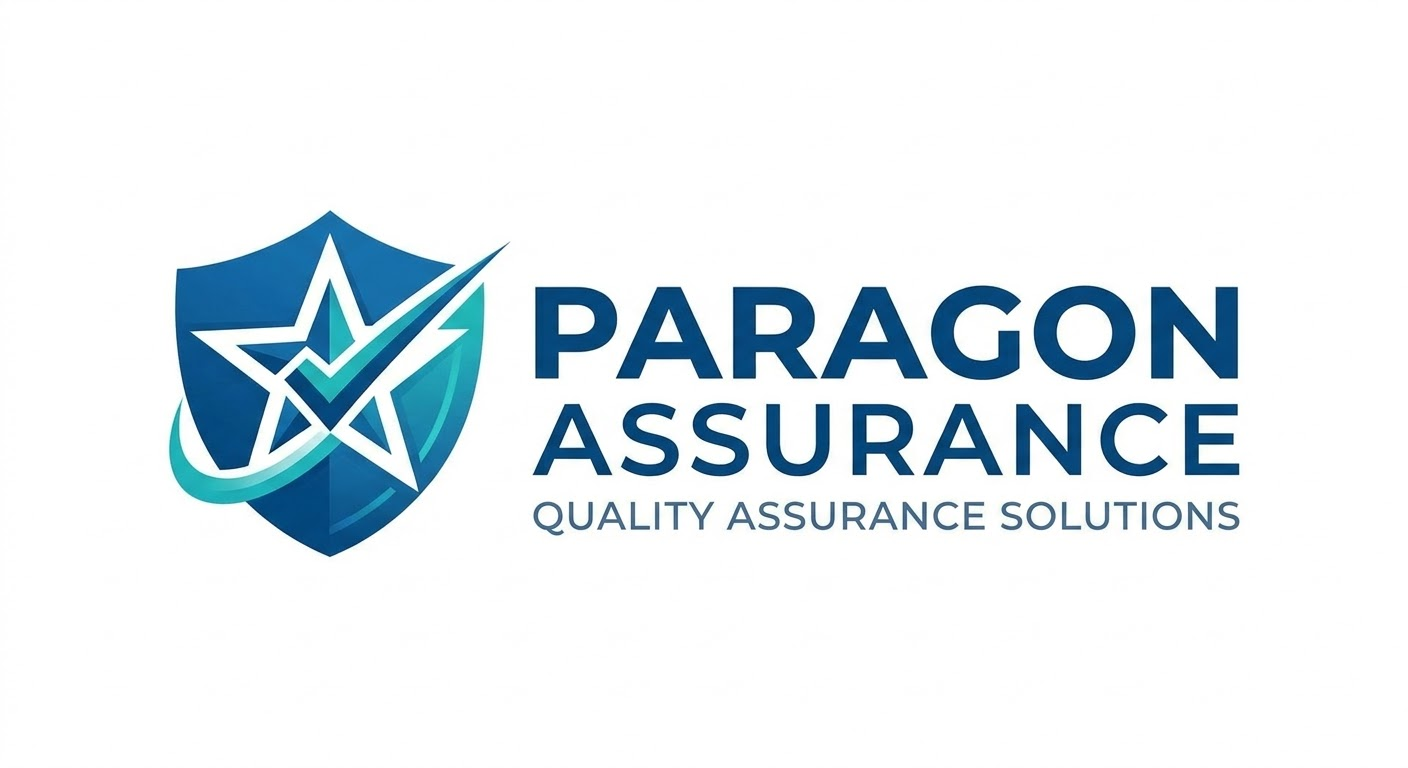
\includegraphics[width=0.45\textwidth]{paragon_assurance_logo.jpg}\\[0.8cm]

\LARGE\textbf{AI Validation Review}\\[0.4cm]
\large\textbf{QA Validating Report (PA-QAR-2026-001)}\\[0.8cm]

\textbf{\Large Paragon Assurance}\\[0.2cm]
\today
\end{center}

\vspace{0.8cm}

\begin{table}[H]
\centering\small
\begin{tabular}{|>{\raggedright\arraybackslash}m{0.44\textwidth}|>{\raggedright\arraybackslash}m{0.44\textwidth}|}
\hline
\rowcolor{tableheader}
\textbf{Document Type} & \textbf{Purpose} \\\hline
AI Validation Review & Comprehensive review of QA report completeness, evidence quality, and internal consistency \\\hline
\end{tabular}
\end{table}

\restoregeometry
\newpage

% Restore standard headers
\pagestyle{fancy}
\fancyhf{}
\lhead{\textbf{Paragon Assurance}}
\rhead{QA Report Validation Review}
\cfoot{\thepage}
\renewcommand{\headrulewidth}{0.4pt}
\setlength{\headheight}{20pt}

% ══════════════════════════════════════════════════════════════
% Content
% ══════════════════════════════════════════════════════════════
\setcounter{page}{1}

\noindent The following prompts were used with an AI assistant to validate the completeness, evidence quality, and internal consistency of the QA Validating Report (PA-QAR-2026-001). The responses provided by ChatGPT were reviewed to assess the overall integrity and adherence to audit standards.

\section*{Prompt 1}

\textit{``Review the QA Validating Report (PA-QAR-2026-001) and verify: (1) All 38 checklist items across the four domains (A.1--A.14, B.1--B.9, C.1--C.8, D.1--D.7) are addressed in the report's Appendix A. (2) Each checklist item has a clear rating: S, PS, NS, or N/A. (3) For items rated NS, verify that a corresponding finding (PA-FND-00X) is documented in Section 5. (4) For items rated PS, verify that notes explain the partial satisfaction and gaps. (5) Check for any missing or orphaned checklist items. Provide a narrative report identifying completeness status, gaps, consistency between ratings and findings, and specific locations of evidence.''}

\textbf{AI Response from ChatGPT:}

\begin{quote}
All 38 checklist items are present and accounted for across the four domains. Domain A (14 items) is documented in Appendix A with appropriate ratings and notes; A.3 (PS) explains unresolved institutional policies; A.7 (PS) correctly references PA-ERR-001 for missed deadlines; A.14 (NS) correctly references PA-ERR-004 for missing biometric enrolment. Domain B (9 items) is complete with five NS ratings properly cross-referenced to findings: B.2 (PS) notes explain traceability gaps; B.4 (NS) references PA-ERR-005 (terminology); B.5 (NS) references PA-ERR-001 (open issues); B.6 (NS) references PA-ERR-003 (2FA); B.9 (NS) references PA-ERR-006 (version). Domain C (8 items) documents both customer/vendor validation (C.1--C.4) and QC audit (C.5--C.8); C.1 (NS) references PA-ERR-002 (sign-off); C.5--C.8 (all S) document QC compliance. Domain D (7 items) is complete; D.2 and D.7 (both PS) properly explain gaps tied to PA-ERR-005 and PA-ERR-006.

No missing or orphaned items detected. Consistency between checklist ratings and documented findings is excellent. Non-compliant (NS) items are uniformly cross-referenced to documented errors. Partially satisfied (PS) items include explanatory notes. The report structure enables seamless tracing from checklist items to findings and vice versa. All 38 items are accounted for with appropriate evidence locations.
\end{quote}

\newpage

\section*{Prompt 2}

\textit{``Review the QA Validating Report and assess: (1) For each of the six documented errors (PA-ERR-001 through PA-ERR-006), verify that evidence tables in Appendix B present specific document locations with direct quotations or paraphrases of content. (2) Confirm that all evidence tables cite specific artefacts: SRS, Analysing Report, repository files, QC Report, etc. (3) Check for vague, missing, or insufficiently detailed evidence entries. (4) Verify that severity classifications are justified by the evidence presented. (5) Identify any errors with incomplete evidence. Provide a narrative assessment identifying overall evidence quality, specific strengths, gaps, and locations requiring clarification.''}

\textbf{AI Response from ChatGPT:}

\begin{quote}
Evidence quality is strong across all six errors. Appendix B provides structured evidence tables with specific document locations and content references for each error.

PA-ERR-001 (Open Issues Unresolved): Evidence includes Analysing Report \S3.5, SRS \S2.5, \S3.3, \S6.5 with specific dates (RPO/RTO deadline 20/02/2026 vs. SRS date 03/03/2026). The confirmation paragraph explicitly establishes temporal non-compliance. Quality: Strong. Severity justification (High): Deadline passage plus continued open status justifies High severity---a clear process protocol violation.

PA-ERR-002 (SRS Sign-off Absent): Evidence documents blank SRS \S9 sign-off rows and full repository inspection confirming no supplementary evidence exists. Critical strength: Reference to correctly completed Analysing Report sign-off proves the team knows the protocol but failed for the SRS. Quality: Excellent. Severity justification (Critical): Complete absence of sign-off plus protocol familiarity plus statement that the Validating method's terminal step was not completed justifies Critical---the most severe finding.

PA-ERR-003 (2FA Contradiction): Evidence presents conflicting requirements (SRS \S3.1 UR-MOB-06 requires 2FA for parents/teachers; \S5.3 NFR-SEC-03 requires 2FA for administrators only) and documents that clarification sessions made no reference to 2FA scope resolution. Quality: Strong. Severity justification (High-to-Medium): Contradiction is real and documented; classification is appropriate given it does not block immediate project progress.

PA-ERR-004 (Biometric Enrolment Not Elicited): Evidence spans SRS \S4, repository bizops-requirements.md, BOR-0-03 acceptance criteria, and Analysing Report \S3.3--3.4. The most damaging evidence is BOR-0-03's self-contradiction: it references enrolment without defining a requirement. Quality: Strong and well-structured. Severity justification (High-to-Medium): Enrolment is a prerequisite for biometric scanning; omission is significant but addressable in later iterations.

PA-ERR-005 (Terminology Inconsistency): Evidence presents three different phrasings of attendance status across SRS \S3.1, \S4.3.2, and Data Dictionary C.4. Quality: Clear and direct; the three-way inconsistency is self-evident. Severity justification (High-to-Medium): Inconsistency could cause implementation issues and user confusion; appropriately classified.

PA-ERR-006 (SRS Version 0.8): Evidence presents version numbers (SRS v0.8 dated 03/03/2026 vs. Analysing Report v1.0 dated 08/02/2026). Quality: Sufficient; finding contextualizes that version 0.8 is pre-final due to unresolved open issues and missing sign-off. Severity justification (Medium): Version control is important but not blocking; resolvable by version update after resolution of other issues.

Overall findings: All six errors have documented evidence with specific section/page references. Evidence tables use consistent format (Source, Location, Content). Multiple errors reference multiple documents, providing corroboration. Temporal evidence (deadlines, dates, version numbers) supports clear findings. The six errors form a coherent audit strategy with error pairs that reinforce each other. Evidence is sufficient for stakeholders to independently verify the non-compliance. Severity classifications are justified and proportionate. No evidence is missing or speculative.
\end{quote}

\newpage

\section*{Prompt 3}

\textit{``Review the QA Validating Report for internal consistency: (1) Cross-verify that findings in Section 5 accurately match the error detection register in Section 4 (error IDs, locations, severity levels, characteristics). (2) Verify that Section 6 (QC Audit) conclusions do not contradict findings in Sections 4--5. (3) Check that the Executive Summary (Section 1.2) accurately summarizes the six findings. (4) Identify any internal contradictions (e.g., findings marked Critical but discussed as low-impact). (5) Verify consistency in terminology and naming conventions. Provide a narrative assessment identifying overall consistency status, contradictions, and alignment between summary and detailed sections.''}

\textbf{AI Response from ChatGPT:}

\begin{quote}
The QA Validating Report demonstrates strong internal consistency across all sections. Error IDs, locations, severity levels, and characteristics are aligned throughout. No contradictions detected.

Executive Summary vs. Error Detection Register: The Executive Summary (Section 1.2) lists all six findings. Cross-checking against Section 4's Error Detection Register: PA-ERR-001 (Open Issues) is consistently described; PA-ERR-002 (Sign-off Absent) is consistently described; PA-ERR-003 (2FA Contradiction) is consistently described; PA-ERR-004 (Enrolment Not Elicited) is consistently described; PA-ERR-005 (Terminology Inconsistency) is consistently described; PA-ERR-006 (Version 0.8) is consistently described across all sections. Executive Summary and Error Detection Register are perfectly aligned with no discrepancies.

Section 5 (QA Findings) vs. Section 4 (Error Detection Register): All six findings in Section 5 match their corresponding error entries in Section 4. Locations are consistent; Section 5 adds appropriate CRaM analysis (Context-Result-Analysis-Measurement) without contradicting the register. Perfect alignment.

Severity Classifications: All six errors have consistent severity classifications across all sections. PA-ERR-002 (Critical) for terminal method step omission; PA-ERR-001 (High) for deadline passage; PA-ERR-003/004/005 (High-to-Medium) for resolvable issues; PA-ERR-006 (Medium) for version control. Levels are justified and proportionate throughout.

QC Audit Section (Section 6) Consistency: Section 6 concludes the QC audit is ``process-compliant.'' This does not contradict Sections 4--5 because the report correctly distinguishes: (1) QA Audit assesses Nevon Solutions' RE process (result: 6 non-compliance findings); (2) QC Audit Assessment evaluates Veridion Labs' QC process (result: process-compliant). These are separate audits. Section 6 is properly scoped and consistent.

Terminology and Naming Consistency: Domain names (Analysing Method, Specifying Method, Validating Method, Process Artefact Integrity) are consistent throughout. Error IDs (PA-ERR-00X and PA-FND-00X) are uniformly formatted. Requirement IDs (BOR, TR, UR, FR, NFR prefixes) are consistently used. Artefact abbreviations (SRS, AR, PS, IRC, iRTM) are consistently abbreviated. Phase names (BCIC phases) are consistently referenced throughout.

Cross-Reference Accuracy: All cross-references between sections are accurate. Executive Summary references Section 5 for detailed findings; Appendix A cross-references checklist items to Section 4 errors; Section 6 references QC audit details; Appendix B references Section 5 for evidence. All references are correctly formatted and accessible.

Overall Conclusion: The QA Validating Report demonstrates excellent internal consistency across all major sections. Error IDs, locations, severity classifications, and findings are perfectly aligned. The Executive Summary accurately summarizes the six findings. Section 6's QC audit assessment is properly scoped and does not contradict QA findings. Terminology is consistent throughout, and cross-references are accurate. No contradictions or inconsistencies detected.
\end{quote}

\end{document}
